\documentclass[parskip=full]{scrartcl}

\usepackage[utf8]{inputenc} % use utf8 file encoding for TeX sources
\usepackage[T1]{fontenc} % avoid garbled Unicode text in pdf
\usepackage[german]{babel} % german hyphenation, quotes, etc
\usepackage{hyperref} % detailed hyperlink/pdf configuration
\usepackage{mathptmx} %Schriftart Times
\usepackage[scaled]{helvet} %
\usepackage{graphicx}
\hypersetup{ % ‘texdoc hyperref‘ for options
pdftitle={Pflichtenheft},
bookmarks=true,
}

\makeatletter
\setlength{\@fptop}{0pt}
\makeatother

\usepackage{csquotes} % provides \enquote{} macro for "quotes"
%TitlePage
{\title{\fontsize{40}{48} \selectfont \textsc{Pflichtenheft-Entwurf}\\
{\fontsize{18}{18} \selectfont Multimediatool zum Testen von Videoencodern}}}
\author {Carina Weber, Jan Benedikt Schwarz, Johannes Werner, Noel Schuhmacher,\\
Sascha Rapp, Simon Grafenhorst}

\begin{document}
\maketitle
\thispagestyle{empty}
\newpage
\tableofcontents
\newpage
\section*{Einleitung}
Vive (lang: Video veritatem) ist ein Programm zum Testen verschiedener Videoencoder. Man hat die Möglichkeit ein Video (mit Filtern) zu bearbeiten welches dann von einem externen Encoder encodiert wird. Dieses encodierte Video kann dann wieder in Vive geladen werden, wo so komfortabel mit graphischen Visualisierungen entschieden werden kann, wie gut der Encoder das Video encodiert hat.
\newpage
\section{Zielbestimmung}
Vive ist ein Multimedia-Framework zum Vergleichen und zur Evaluation von Videoencodern.
\subsection{Musskriterien}
\subsubsection{Rohvideo auswählen und bearbeiten}
\begin{itemize}
\item Video laden
\item Aus einer List von Filtern mehrere Filter auswählen
\item Aus einer List von Artefakten mehrere Artefakte auswählen
\item Filter/Artefakte anpassen
\item Zuvor verwendete Konfigurationen (Filter/Artefakte) auswählen
\item Anzeigen einer Vorschau mit den angewandten Filtern/Artefakten
\item Video abspeichern
\end{itemize}
\subsubsection{Bewerten des Encoders}
\begin{itemize}
\item Das Rohvideo laden
\item Mehrere encodierte Videos laden
\item Bewertungskriterien berrechnen
\item Unterschiede zwischen Roh- und encodiertem Video visualisieren
\item Bewertungskriterien/Videoeigenschaften/Metadaten visualisieren
\item Roh- und encodierte(s) Video(s) nebeneinander synchron abspielen
\end{itemize}
\newpage
\subsubsection{Sonstiges}
\begin{itemize}
\item Zustand des Programms als Projekt speichern
\item Projekt laden
\end{itemize}
\subsection{Wunschkriterien}
\begin{itemize}
\item Encoder integrieren
\item Manuelles Bewertungssystem
\item Pluginsystem für Filter und Artefakte
\item Sich bewegende Artefakte
\item Auswählen von Vorschau Frames
\end{itemize}
\subsection{Abgrenzungskriterien}
\begin{itemize}
\item Die Software ist ausschließlich in englischer Sprache verfügbar
\item Audio wird nicht beachtet
\item Korrektheit der Software wird gewährt bis zu einer Videauflösung von 1980x1020 Pixel
\end{itemize}
\newpage
\section{Produkteinsatz}
Vive soll es Forschungseinrichtungen und Firmen ermöglichen Videoencoder einfach
miteinander zu vergleichen. So kann schnell ein optimaler Encoder für den jeweiligen Zweck
gefunden oder die Qualität eines vorhandenen geprüft werden. Aber auch Privatpersonen können
mit diesem Produkt die Funktionsweise eines Encoders kennenlernen oder einen Encoder für ein
Privatprojekt auswählen.
\subsection{Anwendungsbereiche}
\begin{itemize}
\item Forschungsprojekte
\item Kommerzielle Softwarentwicklung
\item Privatprojekte
\end{itemize}
\subsection{Zielgruppe}
\begin{itemize}
\item Forscher im Bereich Multimedia
\item Videoplattformbetreiber
\item Videobearbeiter
\item Privatanwender
\end{itemize}
\subsection{Betriebsbedingungen}
Die Betriebsbedingungen unterscheiden sich im wesentlichen nicht zu denen normaler Software:
\begin{itemize}
\item Büroumgebung
\item Laufzeiten von bis zu 8h pro Tag sind zu erwarten
\end{itemize}
\newpage
\section{Produktumgebung}

\subsection{Hardware}
\begin{itemize}
\item AMD64 Prozessorarchitektur
\item Intel: Pentium 4 oder neuer
\item AMD: Athlon II, Phenom II oder neuer
\item 5 GB freier Festplattenspeicher
\item Mindestens 4 GB Arbeitsspeicher
\end{itemize}
\subsection{Software}
\begin{itemize}
\item Linux 64 bit (getestet auf Ubuntu)
\item Qt Bibliothek Version 5.5.1
\item Gewünschte Videocodecs
\item ffmpeg 2.7.2 oder höher
\end{itemize}
\newpage


\section{Funktionale Anforderungen}
\subsection{Musskriterien}
\subsubsection{Allgemein}
\textbf{/F0000/ Steuerlemente für Videos}

Videos können mit folgenden Steuerelementen angeschaut werden:
\begin{itemize}
\item Start/Pause-Button
\item Stop-Button
\item Timeline
\item Geschwindigkeitsauswahl:
\begin{itemize}
\item Frame by Frame
\item 0.25x
\item 0.5x
\item 0.75x
\item 1.0x
\item 1.25x
\item 1.5x
\item 1.75x
\item 2.0x
\end{itemize}
\end{itemize}

\textbf{/F0001/ Akzeptierte Rohdateitypen}

\begin{itemize}
\item YUV
\end{itemize}
\newpage
\textbf{/F0002/ Akzeptierte encodede Dateitypen}
\begin{itemize}
\item GStreamer kompatible Dateitypen //TODO
\end{itemize}

\textbf{/F0003/ Anzeigen von Aktionen in Statusleiste}

Folgende Aktionen werden in der Statusleiste angezeigt, falls sie aktiv sind:
\begin{itemize}
\item Anwenden von Filtern/Artefakten
\item Speichern des veränderten Videos
\item Laden der encodierten Videos (also Berrechnung von PSNR,etc.)
\item Speichern des Zustandes des Programms
\item Laden des Zustandes des Programms
\end{itemize}
\subsubsection{Rohvideo auswählen und bearbeiten}
\textbf{/F0100/ Auswahl mit Dateiauswaldialog}

Auswahl eines Videos mit einem Dateiauswahldialog. Erlaubte Dateitypen wie in /F0001/.

\textbf{/F0101/ Angabe von Eigenschaften}
Angabe von
\begin{itemize}
\item Auflösung
\item FPS (Standard:25)
\item Pixelshema
\end{itemize}
um den in /F0001/ spezifizierte Dateityp korrekt einlesen zu können.

\textbf{/F0102/ Erlaubte Pixelshema}
Für das in /F0101/ spezifierte Pixelshema sind folgende Angaben erlaubt:
\begin{itemize}
\item 4:4:4
\item 4:2:2
\item 4:2:0
\item 4:1:1
\end{itemize}

\textbf{/F0103/ Auswahl kürzlich ausgewählter Videos}

Auswahl aus einer Liste mit den 10 zuletzt ausgewählten Videos. Angaben wie in /F0101/ müssen
nicht mehr gemacht werden.

\textbf{/F0104/ Auswahl von Filtern}

Auswahl von einem oder mehreren Filtern, die auf das Video gelegt werden.

\textbf{/F0103/ Filter: Schwarzweiß}

Ein Schwarzweißfilter mit einstellbaren Eigenschaften:
\begin{itemize}
\item Helligkeit
\end{itemize}
\newpage
\textbf{/F0104/ Filter: Unschärfe}

Ein Unschärfefilter mit folgenden einstellbaren Egenschaften:
\begin{itemize}
\item Helligkeit
\item Grad der Unschärfe
\end{itemize}

\textbf{/F0105/ Filter: Farbe}

Ein Farbfilter mit folgenden einstellbaren Eigenschaften:
\begin{itemize}
\item Helligkeit
\item Farbe(n) die herausegefiltert werden sollen
\item Intensität der einzelnen Farben
\end{itemize}

\textbf{/F0106/ Fiter: Kontrast}

Ein Kontrastfilter mit den folgenden einstelbaren Eigenschaften:
\begin{itemize}
\item Helligkeit
\item Stärke des Kontrastes
\end{itemize}

\textbf{/F0107/ Auswahl von Artefakten}

Auswahl von einem oder mehreren Artefakten, die auf das Video gelegt werden.

\textbf{/F0108/ Artefakt: Gittermuster}

Ein Gittermuster mit den folgenden einstellbaren Eigenschaften:
\begin{itemize}
\item Anzahl der vertikalen und horizontalen Linien
\item Farbe
\item Helligkeit
\item Dicke der Linien
\end{itemize}
\newpage
\textbf{/F0109/ Artefakt: Schriftzug}

Ein Schriftzug mit fixer Position und folgenden Eigenschaften:
\begin{itemize}
\item Schriftgröße
\item Farbe
\item Text
\end{itemize}

\textbf{/F0110/ Anwendugsreihenfolge von Filtern/Artefakten}

Ein neu ausgewählter Filter/Artefakte wird ans Ende der Anwendungsreihenfolge angehängt.

\textbf{/F0111/ Ändern der Anwendungsreihenfolge}

Die Anwendungsreihenfolge der Filter/Artefakte kann beliebig geändert werden.

\textbf{/F0112/ Entfernen ausgewählter Filter/Artefakte}

Ausgewählte Filter/Artefakte können wieder entfernt werden.

\textbf{/F0113/ Abspeichern einer Filter/Artefakte Konfiguration}

Abspeichern der Konfiguration von Filtern/Artefakten. Abgespeichert wird:
\begin{itemize}
\item welche Filter/Artefakte ausgewählt wurden
\item die Reihenfolge in der die Filter/Artefakte angewendet werden sollen
\item der jeweilige Zustand, der einstellbaren Eigenschaften der Filter/Artefakte
\end{itemize}

\textbf{/F0114/ Anzeigen einer Vorschau}

Die Vorschau des ausgewählten Videos mit den ausgewählten Filtern und Artefakten besteht aus zwei Stufen:

\textbf{/F0115/ 5 Frame Vorschau}

Jedes mal, wenn der Benutzer etwas an den Artefakten/Filtern ändert, werden 5 Frames aus dem Video sofort gerendert.
\newpage
\textbf{/F0116/ Komplette Vorschau}

Nachdem der Nutzer auf einen entsprechenden Button geklickt hat, kann er das ausgewählte Video mit allen ausgewählten Filtern und Artefakten angeschauen. Steuerelemente wie in /F0000/.

\textbf{/F0117/ Speichern des Videos}

Das veränderte Video kann abgespeichert werden. Das Dateiformat ist dasselbe wie das des Inputvideos.

\textbf{/F0118/ Laden einer Filter/Artefakte Konfiguration}

Gespeicherte Konfigurationen können wieder geladen werden.

\textbf{/F0119/ Alles zurücksetzen}

Ausgewählte Filter und Artefakte können alle auf einmal entfernt werden.
\subsubsection{Encodede Videos bewerten}
\textbf{/F0200/ Encodierte Videos laden}

Laden von mehreren enodierten Videos. Akzeptierte Dteitypen wie in /F0020/.

\textbf{/F0210/ Anzeigen der encodierten Videos}

Die geladenen Videos können angeschaut werden.
\textbf{/F0220/ Anzeigen des Rohvideos}

Das Rohvideo kann angeschaut werden.

\textbf{/F0230/ Steuerelemente}

Alle Videos aus /F0210/ und /F0220/ teilen sich einen Satz Steuerelemente. Steuerlemente wie in /F0000/.
\newpage
\textbf{/F0240/ Anzeigen von Dateiattributen}

Folgende Dateiattribute der Videodateien werden angezeigt:
\begin{itemize}
\item Dateiname
\item Dateigröße
\end{itemize}

\textbf{/F0250/ Anzeigen eines RGB-Histogramms}

Für jedes Video wird ein RGB-Histogramm angezeigt.

\textbf{/F0260/ Anzeigen eines PSNR-Graphen}

Für jedes Video wird ein PSNR-Graph angezeigt.

\textbf{/F0270/ PSNR-Graph als Timeline}

Durch klicken auf den PSNR-Graph wird zu der dazugehörigen Stelle im Video gesprungen (bei allen geladenen Videos wird zu dieser Stelle gesprungen).
\textbf{/F0280/ Farbunterschied zwischen Roh- und encodiertem Video anzeigen}
Anzeigen der Farbdifferenz der einzelnen Farbkanäle zwischen dem Roh- und encodiertem Video.

\textbf{/F0290/ Anzeigen von Makroblöcken}

Falls der Encoder Makroblöcke zum komprimieren verwendet hat, können diese angezeigt werden.

\textbf{/F02100/ Speichern des Zustands}

Der Zustand des Programms  kann gespeichert werden. Gespeichert wird dabei folgendes:
\begin{itemize}
\item Absoluter Pfad zum Rohvideo
\item Absoluter Pfad zu allen geladenen encodierten Videos
\item Aktuelle Abspielstelle in den Videos
\end{itemize}

\textbf{/F02110/ Laden eines Zustandes}

Gespeicherte Zustände können wieder gelden werden.
\subsection{Wunschkriterien}
\textbf{/F1100/ Laden eines Encoders}

Der Encoder, der verwendet werden soll, kann mit einem Dateiauswahldialog ausgewählt werden.

\textbf{/F1110/ Akzeptierte Dateitypen für Encoder}

Akzeptiert werden ELF32,ELF64 Dateien.

\textbf{/F1120/ Encoder interface}

Der Encoder mussüber eine Konsole aufgerufen werden können mit dem Dateinamen zum zu encodierendem Video und verschiedene Encodierungsmodi als Parameter.

\textbf{/F1200/ Spezifizieren von Parametern}

Man kann Parameter angeben, die dem Encoder übergeben werden.

\textbf{/F1210/ Parameterliste}

Mehrere verschiedene Parameter werden in einer Liste zusammengefasst.

\textbf{/F1220/ Mehrfaches aufrufen des Encoders}

Für jeden Eintrag in der Liste aus /F1210/ wird der Encoder aufgerufen.

\textbf{/F1300/ Gewährleistung}

Wenn der Encoder nicht korrekt arbeitet (z.B. nicht terminiert), kann die Korrektheit von Vive nicht grantiert werden.

\textbf{/F1400/ Laden der encodierten Videos}

Wenn alle encodierten Videos erzeugt wurden, werden sie automatisch geladen.
\newpage
\subsubsection{Manuelles Bewertungssystem}
\textbf{/F2100/ Bewerten der encodierten Videos}

Die Qualität eines encodierten Videos kann mit einem 5-Sterne Bewertungssystem bewertet werden.

\textbf{/F2200/ Speichern des Zustandes}

Zusätzlich zu den in /F02100/ spezifizierten Attributen wird die 5-Sterne Bewertung gespeichert.

\textbf{/F2300/ Laden eines Zustandes}

Beim Laden eines Zustandes wie in /F02100/ wird auch die 5-Sterne Bewertung geladen.


\subsubsection{Pluginsystem für Filter und Artefakte}

\textbf{/F3100/ Dynamisches Laden von Plugins}

Beim Programmstart werden Filter und Artefakte dynamisch geladen.



\newpage
\section{Produktdaten}
\subsection{Musskriterien}
\textbf{/D010/ Filter/Artefakt Konfiguration}

Wie in /F0170/ spezifiert:
\begin{itemize}
\item Ausgewählte Filter/Artefakte
\item Reihenfolge der Filter/Artefakte
\item Zustand der einstellbaren Eigenschaften der Filter/Artefakte
\end{itemize}

\textbf{/D020/ Zustand}

Wie in /F02100/ spezifiert:
\begin{itemize}
\item Absoluter Pfad zum Rohvideo
\item Absolute Pfade zu den encodierten Videos
\item Abspielposition der Videos
\end{itemize}

\textbf{/D030/ Zuletzt ausgewählte Videos}

Wie in /F0110/ spezifiert:
\begin{itemize}
\item Absoute Pfade zu den 10 zuletzt ausgewählten Videos
\end{itemize}

\subsection{Wunschkriterien}
\textbf{/D110/ 5-Sterne Bewertung}

Die manuelle Bewertung, wie in /F2200? spezifiziert.


\newpage
\section{Nichtfunktionale Anforderungen}
\textbf{/L010/ Responsive GUI}

Auch bei rechenintensiven Hintergrundaktionen bleibt die GUI responsive.

\textbf{/L020/ Fehlerrobust}

Bei Fehlerhaften Videodateien oder Nutzereingaben soll das Programm nicht abstürzen.
\newpage
\section{Benutzungsoberflächer}
\subsection{Anforderungen}
Die Bedienungsoberfläche ist auf Mausbedienung ausgelegt, eine Bedienung ohne Maus muss dennoch möglich sein.
\begin{itemize}
\item DIN 66234, Teil 8 ist zu beachten
\item Die Benutzungsoberfläche wird aus Elementen des Qt Designer aufgebaut
\end{itemize}
\subsection{Beispieldesign}

\subsubsection{Videoauswahl}
\begin{figure}[htbp] 
\centering
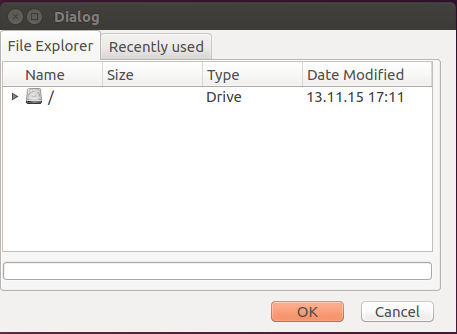
\includegraphics[width=0.7\textwidth]{ToViET/Screenshots/Explorer.png}
\caption{Videoauswahl}
\end{figure}
\newpage
\subsubsection{Filter/Artefakte}
\begin{figure}[htbp] 
\centering
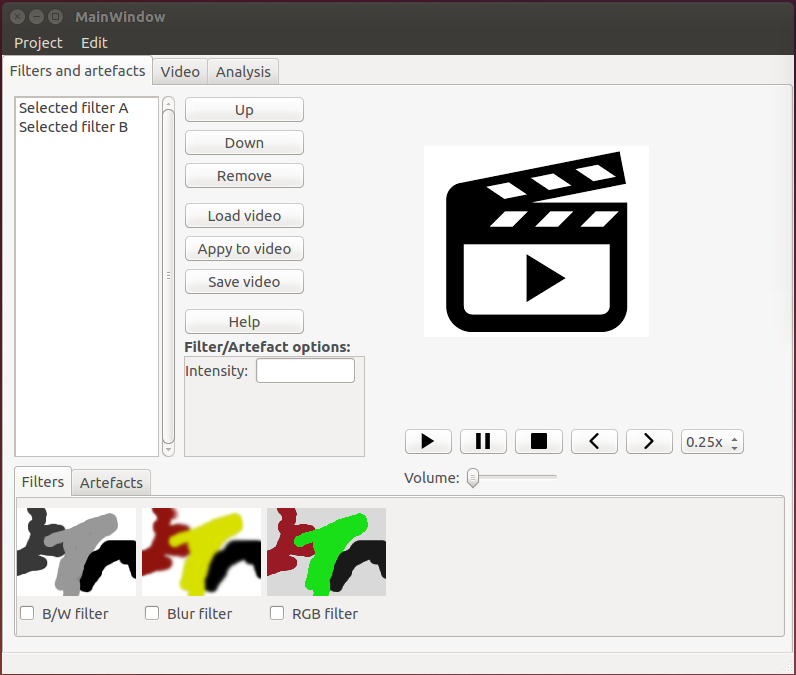
\includegraphics[width=0.7\textwidth]{ToViET/Screenshots/MainWindow_1.png}
\caption{Filter/Artefakte Auswahl}
\end{figure}
\newpage
\subsubsection{Wiedergabe und Auswertung}
\begin{figure}[htbp]
\centering
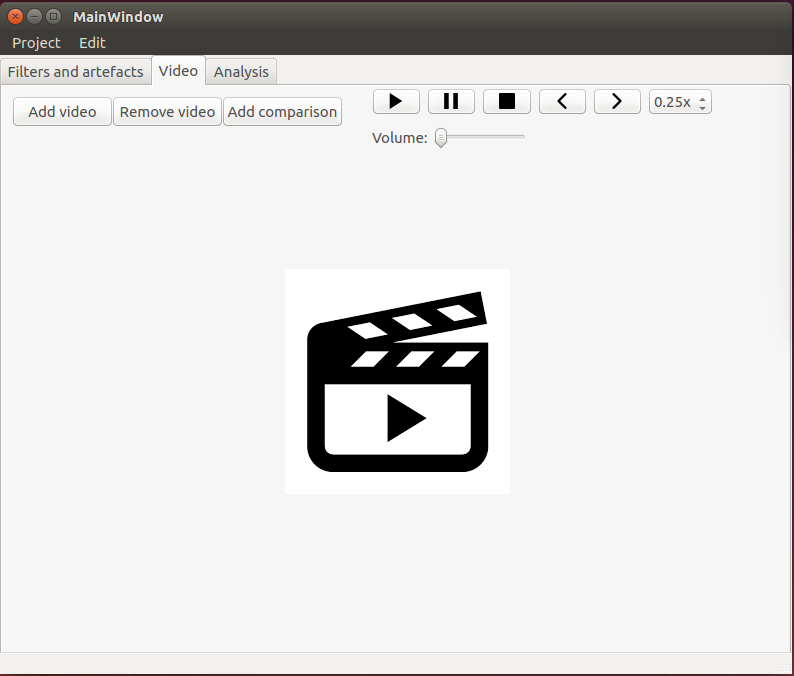
\includegraphics[width=0.5\textwidth]{ToViET/Screenshots/MainWindow_3.png}
\caption{Wiedergabe und Auswertung}
\end{figure}
\begin{figure}[htbp]
\centering
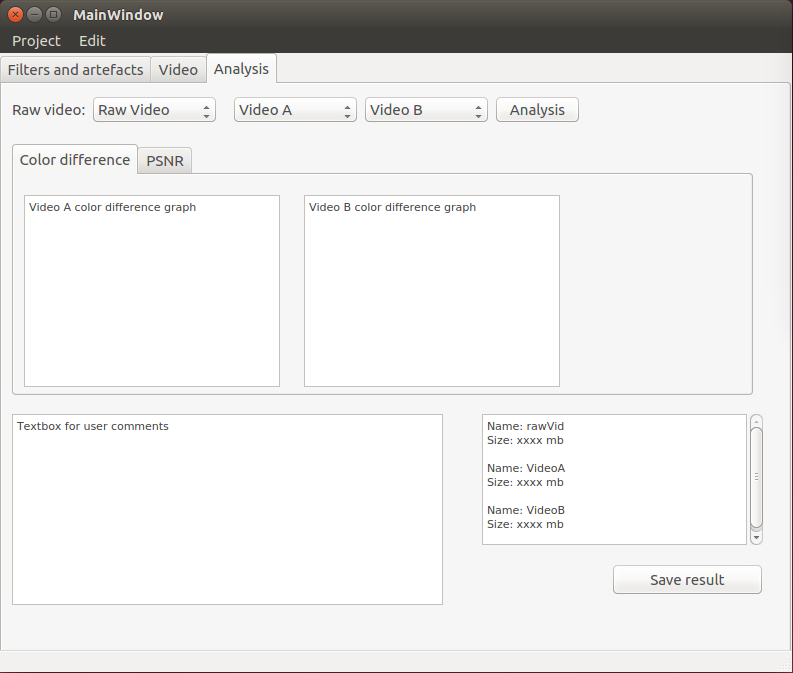
\includegraphics[width=0.5\textwidth]{ToViET/Screenshots/MainWindow_4.png}
\caption{Wiedergabe und Auswertung}
\end{figure}
\newpage
\section{Qualitätsbestimmungen}
\begin{tabular}{|c|c|c|c|c|}
\hline & Sehr wichtig & Wichtig & Weniger wichtig & Unwichtig \\
\hline Robustheit & • &  &  & \\ 
\hline Zuverlässigkeit & • &  &  & \\ 
\hline Korrektheit & • &  &  & \\ 
\hline Benutzerfreundlichkeit & • &  &  & \\ 
\hline Effizienz &  & • &  & \\ 
\hline Portierbarkeit &  &  & • & \\ 
\hline Kompatibilität &  &  & • & \\ 
\hline Modifizierbarkeit &  &  & • & \\ 
\hline Sicherheit &  &  &  & • \\ 
\hline 
\end{tabular} 
\newpage
\section{Systemmodelle}
\begin{figure}[htbp]
\centering
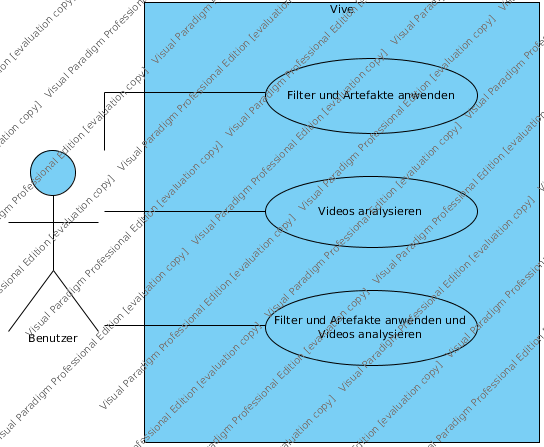
\includegraphics[width=0.7\textwidth]{UsecaseDiagrams/Vive.png}
\caption{Komplettes Programm}
\begin{flushleft}
Das Programm bietet zwei getrennte Funktionalitäten. Der Benutzer kann Filter und Artefakte auf eine Videosequenz anwenden und/oder mehrere Videos analysieren.
\end{flushleft}
\end{figure}
\begin{figure}[htbp]
\centering
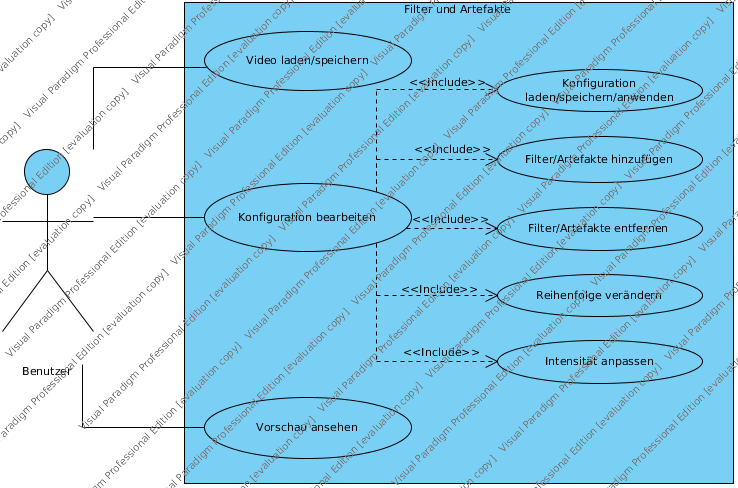
\includegraphics[width=0.7\textwidth]{UsecaseDiagrams/Filter_und_Artefakte.png}
\caption{Filter und Artefakte}
\begin{flushleft}
Während des Anwendens der Filter und Artefakte hat der Benutzer die Möglichkeit ein Video zu laden/speichern, die aktuelle Konfiguration zu bearbeiten und sich eine Vorschau anzeigen zu lassen. Das Bearbeiten der Konfiguration beinhaltet das Laden/Speichern/Anwenden der aktuellen Konfiguration, das Hinzufügen/Entfernen von Filtern und Artefakten, sowie das Verändern ihrer Reihenfolge. Zudem können Parameter wie die Intensität jedes Filters und Artefakts angepasst werden.
\end{flushleft}
\end{figure}
\begin{figure}[htbp]
\centering
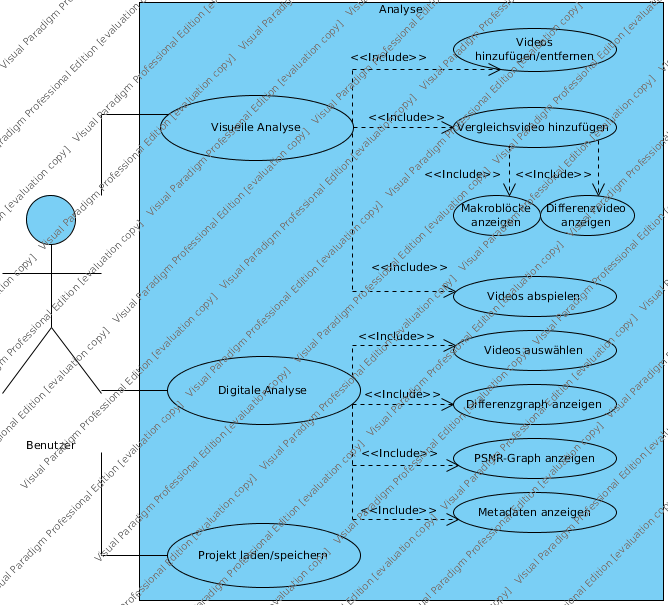
\includegraphics[width=0.7\textwidth]{UsecaseDiagrams/Analyse.png}
\caption{Videoanalyse}
\begin{flushleft}
Der Benutzer hat die Möglichkeit mehrere Videos sowohl subjektiv als auch objektiv zu analysieren. Für die subjektive Analyse kann er Videos zur Übersicht hinzufügen, abspielen und wieder entfernen. Zudem kann er Differenzvideos hinzufügen oder Makroblocks ansehen.
Zur objektiven Analyse können PSNR-Graphen, Bitrate-Graphen und Differenzgraphen angezeigt werden.
Der Zustand des Projekts kann jederzeit gespeichert und geladen werden.
\end{flushleft}
\end{figure}
\newpage
\section{Globale Testfälle und Szenarien}
\subsection{Testfälle}
Folgende Funktionssequenzen sind zu überprüfen:
\begin{itemize}
\item[]\textbf{/T000/}\qquad Oben auf "'Project"' und dann auf "'new"' klicken.
\item[]\textbf{/T001/}\qquad Zwischen den Tabs wechseln.
\item[]\textbf{/T002/}\qquad Auf dem Video Tabs auf "'Add video"' klicken.
\item[]\textbf{/T003/}\qquad "'Load video"' klicken und unter "'File Explorer"' ein Video auswählen.
\item[]\textbf{/T004/}\qquad "'Load video"' klicken und unter "'Recent used"' ein Video auswählen.
\item[]\textbf{/T005/}\qquad Filter auswählen und deren Reihenfolge und Intensity ändern.
\item[]\textbf{/T006/}\qquad Artefakte auswählen und deren Reihenfolge  ändern.
\item[]\textbf{/T007/}\qquad Filter/Artefakte auswählen und "'Apply to video"' klicken.
\item[]\textbf{/T008/}\qquad laden Filter/Artefakte auswählen und Vorschau des Videos testen.
\item[]\textbf{/T009/}\qquad laden Filter/Artefakte auswählen und "'Save video"' klicken.
\item[]\textbf{/T010/}\qquad Auf "'Remove video"' klicken.
\item[]\textbf{/T011/}\qquad Mehrere Videos durch "'Add video"' aufrufen.
\item[]\textbf{/T012/}\qquad Videos mit verschiedenen Geschwindigkeit abspielen.
\item[]\textbf{/T013/}\qquad Videos mit < und > und Frame für Frame  durchgehen.
\item[]\textbf{/T014/}\qquad Videos Starten, Pausieren und Stoppen.
\item[]\textbf{/T015/}\qquad Ergebnisse der Analysis betrachten.
\item[]\textbf{/T016/}\qquad Comment schreiben und auf "'Save result"' klicken.
\item[]\textbf{/T017/}\qquad Oben auf "'Edit"' und dann auf "'undo"'/"'redo"' klicken.
\item[]\textbf{/T018/}\qquad Oben auf "'Project"' und dann auf "'Save"'/"'Save As"' klicken.
\item[]\textbf{/T019/}\qquad Oben auf "'Project"' und dann auf "'Load"' klicken.
\end{itemize}
\subsection{Szenarien}
Folgende Szenarien sind zu überprüfen:
\begin{itemize}
\item[]\textbf{/T100/}\qquad Der Benutzer startet zunächst ein neues Project und fügt dann ein Rohvideo hinzu, indem er auf "'Add video"' klickt. Daraufhin fügt er durch klicken von "'Add video"' eine encodierte Version des Videos hinzu. Bei diesen betrachtet er dann die Video zunächst mit 0.5x, 1.0x, 1.5x facher Geschwindigkeit und geht die Videos dann "frame by frame" durch. Dann betrachtet er den PSNR Graphen und die Makroblöcke sowie weitere Analyse Auswertungen. Zuletzt schreibt er ein Kommentar in das "'User comment"' Feld und speichert dann die Analysis durch drücken von "'Save result"' und das Project durch drücken von "'Save as"' oben unter Project.
\item[]\textbf{/T101/}\qquad Der Benuter startet ein neues Project. Dann lädt er im "'Filters and artefacts"' Tab ein Video und wählt mehrere Filter/ Artefakte aus. Daraufhin verändert er die Reihenfolge der Filter/ Artefakteund speichert das Video ab. Nachdem er das abgespeicherte Video encodiert hat fügt er dieses zusammen mit dem Rohvideo als neues Video im "'Video"' Tab hinzu. Danach betrachtet er die Videos und die dazugehörigen Analyse Auswertungen. zuletzt speichert er das Ergebnisse mit einem Kommentar ab.
\item[]\textbf{/T102/}\qquad Der Benutzer lädt ein bereits existierendes Project durch klicken auf Project und Load. Er betrachtet dann die geladenen Videos und deren Analyse Auswertungen. Daraufhin schaut er sich unter dem "'Filters and artefacts"' Tab die ausgewählten Filter des zuletzt bearbeiteten Videos an. Danach schließt er das Programm.
\end{itemize}
\newpage
\section{Glossar}
\subsection*{5-Sterne Bewertungssystem}  
5 Sterne zur Bewertung, wobei 1 Stern die niedrigste Bewertung ist und 5 Sterne die höchste.

\subsection*{Artefakt} Eine Struktur, die über das Video gelegt wird, wie zum Beispiel ein Kreis oder eine Linie.
\subsection*{Benutzer} 
Weibliche oder männliche Person, die das Programm benutzt.
\subsection*{Encoder} 
Ein Programm zum komprimieren von Videodateien.
\subsection*{Filter} 
Ein Algorithmus, der Farbwerte nach einem bestimmten Muster verändert.
\subsection*{Frame}
Ein einziges Bild aus einem Video
\subsection*{Projekt} 
Ein Projekt beinhaltet die Pfade zu den geöffneten Videos sowie die eingestellten Filter und Artefakte.
\subsection*{PSNR-Graph} 
Ein Graph der auf der x-Achse Zeitwerte(Framenummer) enthält und auf der y-Achse den dazugehörigen PSNR-Wert.
\subsection*{PSNR-Wert} 
Peak signal-to-noise ratio ist ein Maß für das Verhältnis zwischen Signalrate und dem überlagerten Rauschsignal.
\subsection*{RGB-Histogramm} 
Ein Graph, der die Farbverteilung eines Videos anzeigt.
\subsection*{Tab\ (Deutsch: Registerkarte)}
Graphische Elemente die dazu dienen in einem Fenster zwischen verschiedenen Dialogfenstern zu wechseln.
\end{document}